\documentclass[11pt,a4paper]{report}
\usepackage[textwidth=37em,vmargin=30mm]{geometry}
\usepackage{calc,xunicode,amsmath,amssymb,paralist,enumitem,tabu,booktabs,datetime2,xeCJK,xeCJKfntef,listings}
\usepackage{tocloft,fancyhdr,tcolorbox,xcolor,graphicx,eso-pic,xltxtra,xelatexemoji}

\newcommand{\envyear}[0]{2024}
\newcommand{\envdatestr}[0]{2024-11-13}
\newcommand{\envfinaldir}[0]{webdb/2024/20241113/final}

\usepackage[hidelinks]{hyperref}
\hypersetup{
    colorlinks=false,
    pdfpagemode=FullScreen,
    pdftitle={Web Digest - \envdatestr}
}

\setlength{\cftbeforechapskip}{10pt}
\renewcommand{\cftchapfont}{\rmfamily\bfseries\large\raggedright}
\setlength{\cftbeforesecskip}{2pt}
\renewcommand{\cftsecfont}{\sffamily\small\raggedright}

\setdefaultleftmargin{2em}{2em}{1em}{1em}{1em}{1em}

\usepackage{xeCJK,xeCJKfntef}
\xeCJKsetup{PunctStyle=plain,RubberPunctSkip=false,CJKglue=\strut\hskip 0pt plus 0.1em minus 0.05em,CJKecglue=\strut\hskip 0.22em plus 0.2em}
\XeTeXlinebreaklocale "zh"
\XeTeXlinebreakskip = 0pt


\setmainfont{Brygada 1918}
\setromanfont{Brygada 1918}
\setsansfont{IBM Plex Sans}
\setmonofont{JetBrains Mono NL}
\setCJKmainfont{Noto Serif CJK SC}
\setCJKromanfont{Noto Serif CJK SC}
\setCJKsansfont{Noto Sans CJK SC}
\setCJKmonofont{Noto Sans CJK SC}

\setlength{\parindent}{0pt}
\setlength{\parskip}{8pt}
\linespread{1.15}

\lstset{
	basicstyle=\ttfamily\footnotesize,
	numbersep=5pt,
	backgroundcolor=\color{black!5},
	showspaces=false,
	showstringspaces=false,
	showtabs=false,
	tabsize=2,
	captionpos=b,
	breaklines=true,
	breakatwhitespace=true,
	breakautoindent=true,
	linewidth=\textwidth
}






\newcommand{\coverpic}[2]{
    % argv: itemurl, authorname
    Cover photo by #2~~(\href{#1}{#1})
}
\newcommand{\makeheader}[0]{
    \begin{titlepage}
        % \newgeometry{hmargin=15mm,tmargin=21mm,bmargin=12mm}
        \begin{center}
            
            \rmfamily\scshape
            \fontspec{BaskervilleF}
            \fontspec{Old Standard}
            \fontsize{59pt}{70pt}\selectfont
            WEB\hfill DIGEST
            
            \vfill
            % \vskip 30pt
            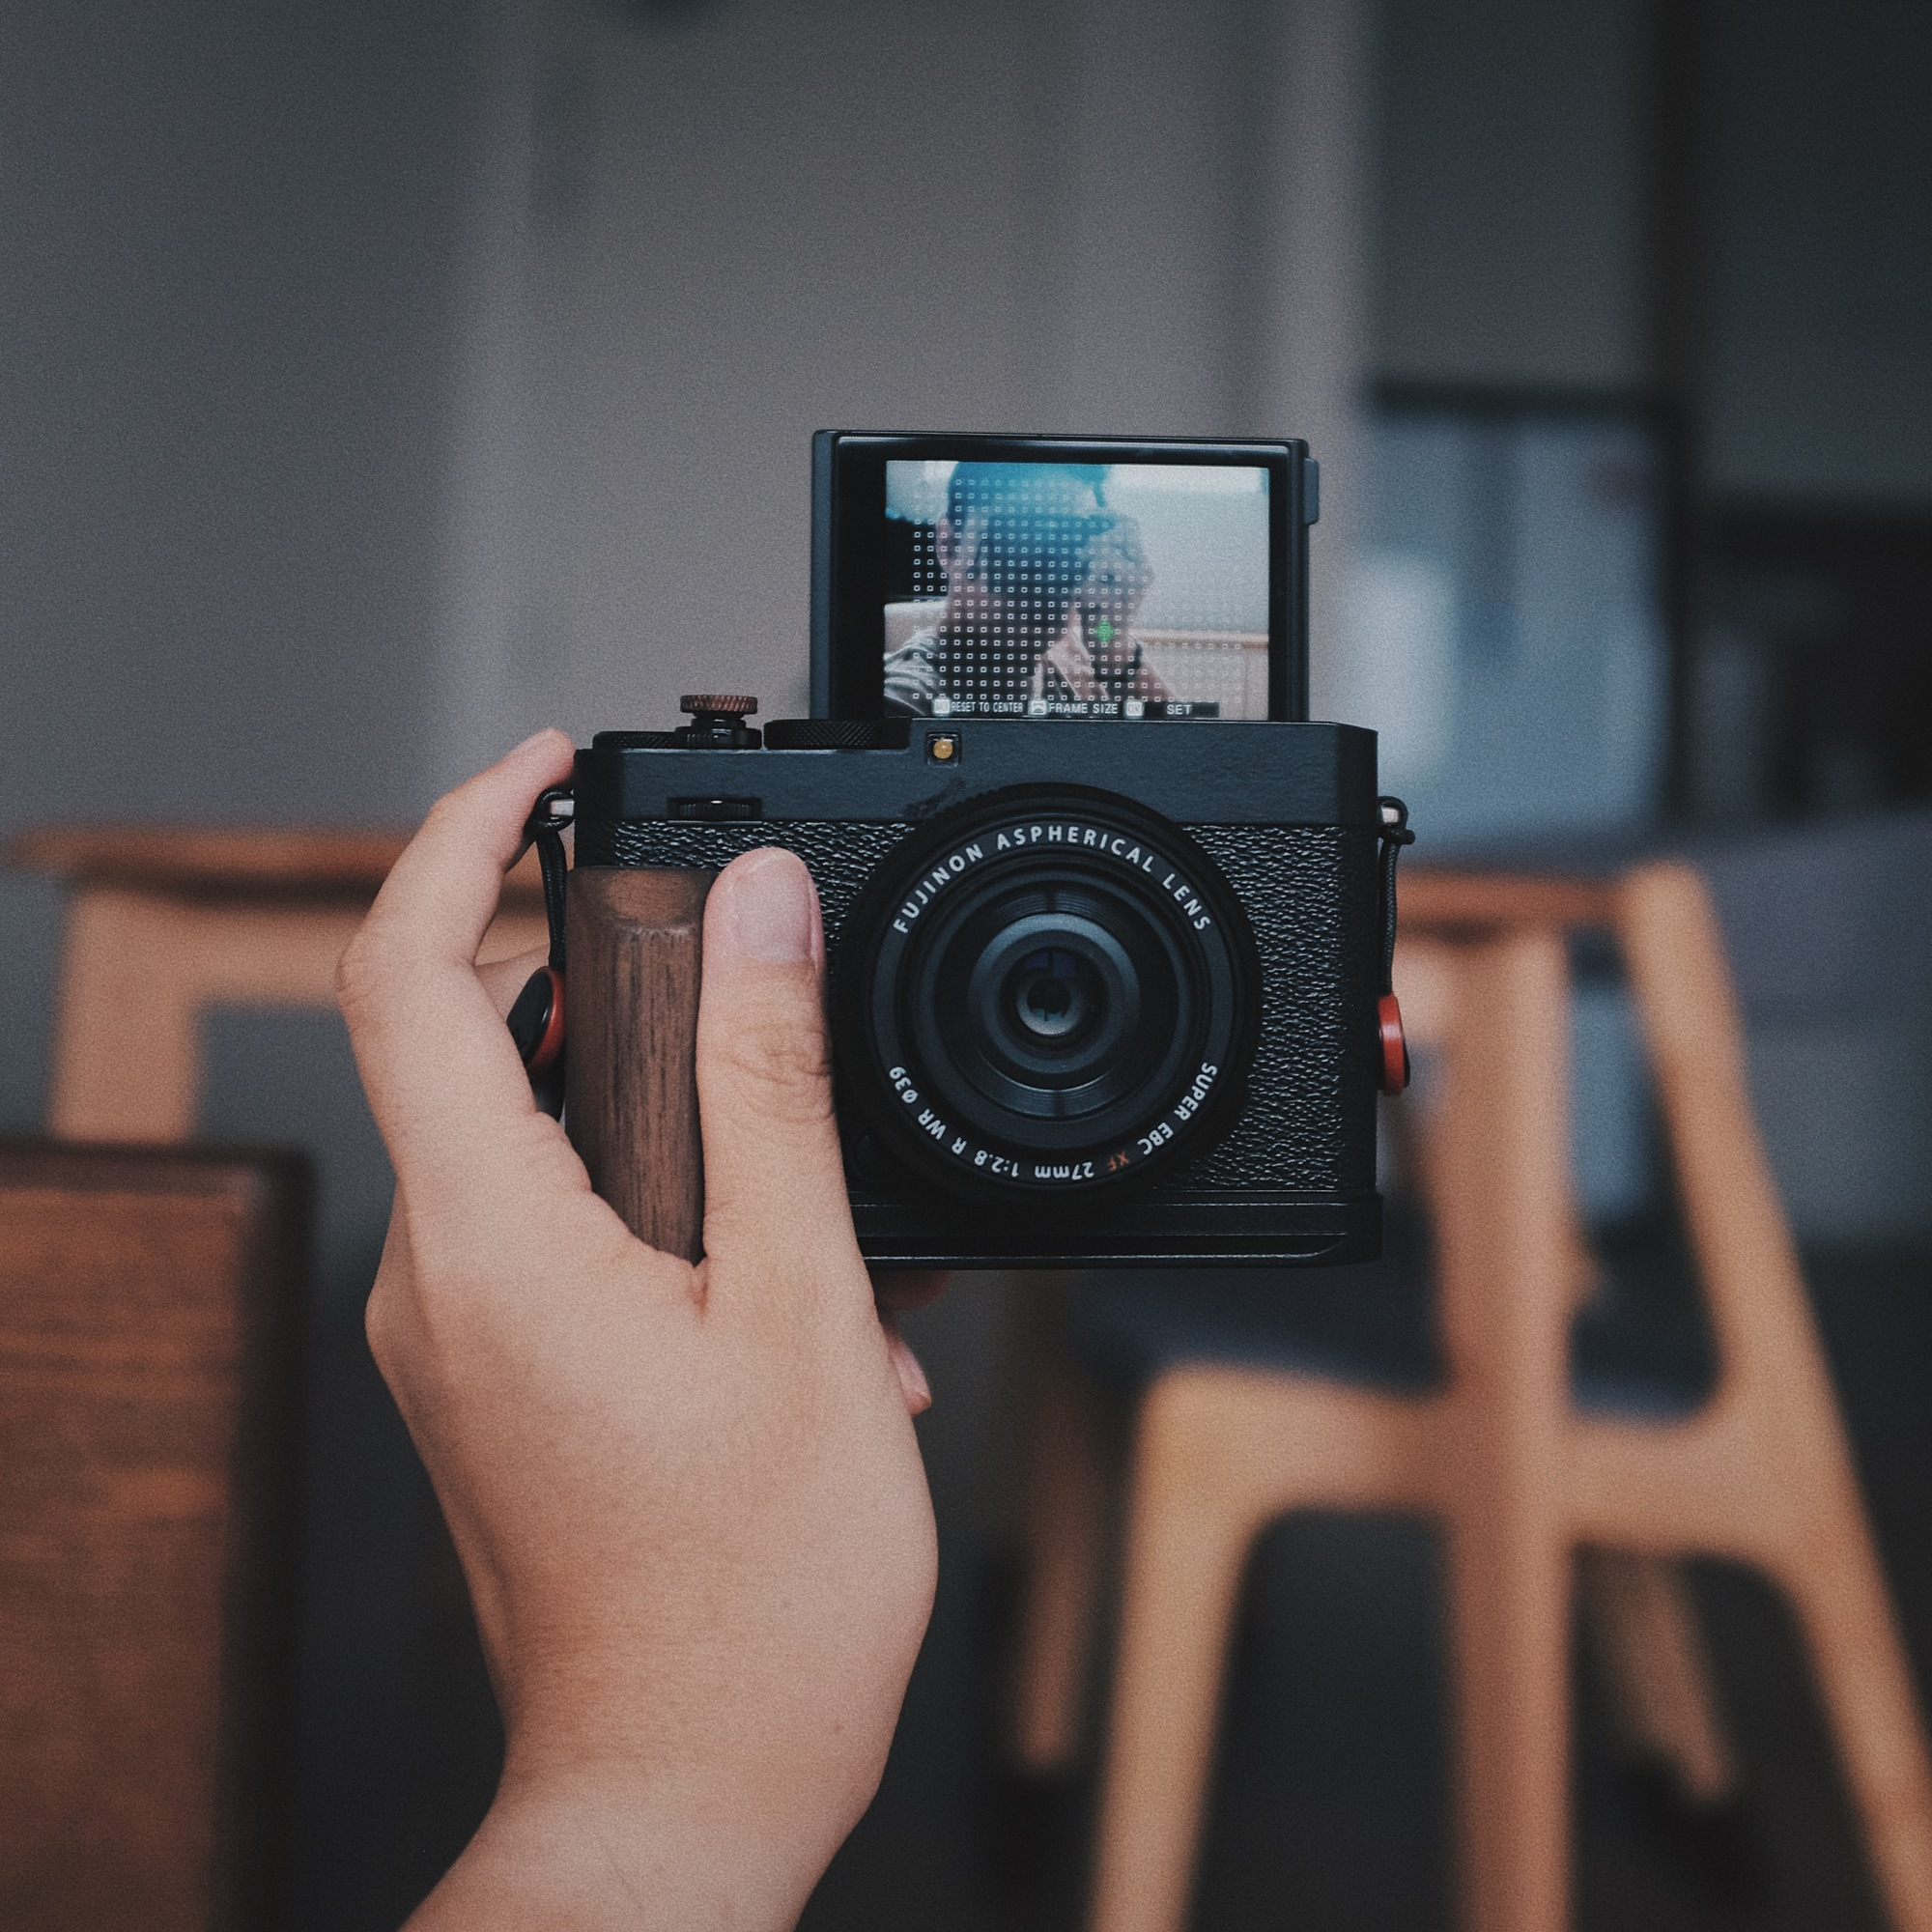
\includegraphics[width=\linewidth]{\envfinaldir/coverpic-prod.jpg}\par
            % \vskip 30pt
            \vfill

            \normalsize\rmfamily\scshape
            \copyright{} The Web Digest Project \hfill\large \envdatestr
        \end{center}
    \end{titlepage}
    % \restoregeometry
}
\newcommand{\simplehref}[1]{%
    \textcolor{blue!80!green}{\href{#1}{#1}}%
}
\renewcommand{\contentsname}{\center\Huge\sffamily\bfseries Contents\par\vskip 20pt}
\newcounter{ipartcounter}
\setcounter{ipartcounter}{0}
\newcommand{\ipart}[1]{
    % \vskip 20pt
    \clearpage
    \stepcounter{ipartcounter}
    \phantomsection
    \addcontentsline{toc}{chapter}{#1}
    % \begin{center}
    %     \Huge
    %     \sffamily\bfseries
    %     #1
    % \end{center}
    % \vskip 20pt plus 7pt
}
\newcounter{ichaptercounter}
\setcounter{ichaptercounter}{0}
\newcommand{\ichapter}[1]{
    % \vskip 20pt
    \clearpage
    \stepcounter{ichaptercounter}
    \phantomsection
    \addcontentsline{toc}{section}{\numberline{\arabic{ichaptercounter}}#1}
    \begin{center}
        \Huge
        \sffamily\bfseries
        #1
    \end{center}
    \vskip 20pt plus 7pt
}
\newcommand{\entrytitlefont}[1]{\subsection*{\raggedright\Large\sffamily\bfseries#1}}
\newcommand{\entryitemGeneric}[2]{
    % argv: title, url
    \parbox{\linewidth}{
        \entrytitlefont{#1}\par\vskip 5pt
        \footnotesize\ttfamily\mdseries
        \simplehref{#2}
    }\vskip 11pt plus 11pt minus 1pt
}
\newcommand{\entryitemGithub}[3]{
    % argv: title, url, desc
    \parbox{\linewidth}{
        \entrytitlefont{#1}\par\vskip 5pt
        \footnotesize\ttfamily\mdseries
        \simplehref{#2}\par\vskip 5pt
        \small\rmfamily\mdseries#3
    }\vskip 11pt plus 11pt minus 1pt
}
\newcommand{\entryitemAp}[3]{
    % argv: title, url, desc
    \parbox{\linewidth}{
        \entrytitlefont{#1}\par\vskip 5pt
        \footnotesize\ttfamily\mdseries
        \simplehref{#2}\par\vskip 5pt
        \small\rmfamily\mdseries#3
    }\vskip 11pt plus 11pt minus 1pt
}
\newcommand{\entryitemHackernews}[3]{
    % argv: title, hnurl, rawurl
    % \parbox{\linewidth}{
    %     \entrytitlefont{#1}\par\vskip 5pt
    %     \footnotesize\ttfamily\mdseries
    %     \simplehref{#3}\par
    %     \textcolor{black!50}{\href{#2}{#2}}
    % }\vskip 11pt plus 11pt minus 1pt
    \begin{minipage}{\linewidth}
            \entrytitlefont{#1}\par\vskip 5pt
            \footnotesize\ttfamily\mdseries
            \simplehref{#3}\par
            \textcolor{black!50}{\href{#2}{#2}}
    \end{minipage}\par\vskip 11pt plus 11pt minus 1pt
}







\begin{document}

\makeheader

\tableofcontents\clearpage




\ipart{Developers}
\ichapter{Hacker News}
\entryitemTwoLinks{M4 Mac mini's efficiency}{https://news.ycombinator.com/item?id=42120311}{https://www.jeffgeerling.com/blog/2024/m4-mac-minis-efficiency-incredible}

\entryitemTwoLinks{Mom jailed for letting 10-year-old walk alone to town}{https://news.ycombinator.com/item?id=42118970}{https://reason.com/2024/11/11/mom-jailed-for-letting-10-year-old-walk-alone-to-town/}

\entryitemTwoLinks{Visualizing 13M Bluesky users}{https://news.ycombinator.com/item?id=42118180}{https://joelgustafson.com/posts/2024-11-12/vizualizing-13-million-bluesky-users}

\entryitemTwoLinks{Waymo One is now open to all in Los Angeles}{https://news.ycombinator.com/item?id=42117008}{https://waymo.com/blog/2024/11/waymo-one-open-to-all-in-los-angeles/}

\entryitemTwoLinks{A neurology ICU nurse on AI in hospitals}{https://news.ycombinator.com/item?id=42115873}{https://www.codastory.com/stayonthestory/nursing-ai-hospitals-robots-capture/}

\entryitemTwoLinks{The EdTech Revolution Has Failed}{https://news.ycombinator.com/item?id=42115597}{https://www.afterbabel.com/p/the-edtech-revolution-has-failed}

\entryitemTwoLinks{Two upstart search engines are teaming up to take on Google}{https://news.ycombinator.com/item?id=42114990}{https://www.wired.com/story/ecosia-qwant-eusp-take-on-google-search-index/}

\entryitemTwoLinks{Cheaper to rent in Barcelona and commute to London (2013)}{https://news.ycombinator.com/item?id=42113479}{https://bestburgerinnorthwestlondon.wordpress.com/2013/10/24/cheaper-to-rent-in-barcelona-and-commute-to-london/}

\entryitemTwoLinks{Bluesky adds 700k new users in a week}{https://news.ycombinator.com/item?id=42112432}{https://www.theverge.com/2024/11/11/24293920/bluesky-700000-new-users-week-x-threads}

\entryitemTwoLinks{What I wish someone told me about Postgres}{https://news.ycombinator.com/item?id=42111896}{https://challahscript.com/what\_i\_wish\_someone\_told\_me\_about\_postgres}

\entryitemTwoLinks{Bus Number – The GitHub plugin my coworkers asked me not to write}{https://news.ycombinator.com/item?id=42111260}{https://www.scannedinavian.com/the-github-plugin-my-coworkers-asked-me-not-to-write.html}

\entryitemTwoLinks{Misguided Apple Intelligence ads}{https://news.ycombinator.com/item?id=42111094}{https://tidbits.com/2024/11/11/misguided-apple-intelligence-ads/}

\entryitemTwoLinks{How I ship projects at big tech companies}{https://news.ycombinator.com/item?id=42111031}{https://www.seangoedecke.com/how-to-ship/}

\entryitemTwoLinks{I Don't Have Spotify}{https://news.ycombinator.com/item?id=42110877}{https://github.com/sjdonado/idonthavespotify}

\entryitemTwoLinks{Improving Steam Client Stability on Linux}{https://news.ycombinator.com/item?id=42110677}{https://ttimo.typepad.com/blog/2024/11/the-steam-client-update-earlier-this-week-mentions-fixed-some-miscellaneous-common-crashes-in-the-linux-notes-which-i-wante.html}

\entryitemTwoLinks{The online sports gambling experiment}{https://news.ycombinator.com/item?id=42110194}{https://thezvi.substack.com/p/the-online-sports-gambling-experiment}

\entryitemTwoLinks{Every arthouse buff you know is pirating films}{https://news.ycombinator.com/item?id=42109544}{https://i-d.co/article/streaming-arthouse-movies-john-waters-netflix-2024/}

\entryitemTwoLinks{The death and life of prediction markets at Google}{https://news.ycombinator.com/item?id=42108360}{https://asteriskmag.com/issues/08/the-death-and-life-of-prediction-markets-at-google}

\entryitemTwoLinks{The business of gutting failed Bay Area tech companies}{https://news.ycombinator.com/item?id=42107870}{https://www.sfgate.com/bayarea/article/better-source-cheap-bay-area-office-furniture-19897542.php}

\entryitemTwoLinks{Did scientists revive an extinct animal or just breed a less stripey zebra?}{https://news.ycombinator.com/item?id=42107534}{https://www.wsj.com/science/biology/quagga-woolly-mammoth-extinct-zebra-africa-dabce258}\ichapter{Phoronix}
\entryitemGeneric{\hskip 0pt{}Intel Idle Support For Granite Rapids D Going Into Linux 6.13}{https://www.phoronix.com/news/Intel-Idle-Granite-Rapids-D}

\entryitemGeneric{\hskip 0pt{}Intel Releases New CPU Microcode For Two New Security Advisories}{https://www.phoronix.com/news/Intel-November-2024-CPU-Micro}

\entryitemGeneric{\hskip 0pt{}Early Benchmarks: AMD EPYC 9005 Performance \& Power Efficiency To Lead Further With Linux 6.13}{https://www.phoronix.com/review/amd-epyc-9005-pstate}

\entryitemGeneric{\hskip 0pt{}GNOME Mutter Lands Improved GPU Selection Logic For Laptops}{https://www.phoronix.com/news/GNOME-Mutter-Multi-GPU-eDP}

\entryitemGeneric{\hskip 0pt{}Red Hat Acquiring Neural Magic To Bolster Open-Source AI Offerings}{https://www.phoronix.com/news/Red-Hat-Neural-Magic}

\entryitemGeneric{\hskip 0pt{}Mesa 25.0 Clover OpenCL Drops Support For NIR Drivers}{https://www.phoronix.com/news/Mesa-25.0-Clover-Drops-NIR}

\entryitemGeneric{\hskip 0pt{}AMD's Ninth Iteration Of Their XDNA Linux Driver Posted For Ryzen AI}{https://www.phoronix.com/news/AMD-XDNA-Linux-Driver-v9}

\entryitemGeneric{\hskip 0pt{}Red Hat \& Intel Developing "Climatik" For Power Capping AI In The Data Center}{https://www.phoronix.com/news/Red-Hat-Climatik}

\entryitemGeneric{\hskip 0pt{}GCC 15 Lands New Optimization For AMD Zen 4 \& Zen 5 CPUs}{https://www.phoronix.com/news/GCC-AVX512-Two-Epi-AMD-Zen-5}


\ipart{Developers~~~~(zh-Hans)}
\ichapter{Solidot}
\entryitemGeneric{\hskip 0pt{}俄罗斯的可重复使用火箭计划}{https://www.solidot.org/story?sid=79755}

\entryitemGeneric{\hskip 0pt{}Firefox 将人和隐私置于利润之上}{https://www.solidot.org/story?sid=79754}

\entryitemGeneric{\hskip 0pt{}Google 要求 Android 芯片组支持 Virtualization Framework }{https://www.solidot.org/story?sid=79753}

\entryitemGeneric{\hskip 0pt{}Ilya Sutskever 认为大模型规模已经达到平台期}{https://www.solidot.org/story?sid=79752}

\entryitemGeneric{\hskip 0pt{}双 11 购物节没有恢复往日的火热}{https://www.solidot.org/story?sid=79751}

\entryitemGeneric{\hskip 0pt{}病毒学家用其在实验室培养的病毒治疗自己的癌症}{https://www.solidot.org/story?sid=79750}

\entryitemGeneric{\hskip 0pt{}亚马逊证实员工信息泄露}{https://www.solidot.org/story?sid=79749}

\entryitemGeneric{\hskip 0pt{}FTX 起诉币安及其前 CEO 赵长鹏}{https://www.solidot.org/story?sid=79748}

\entryitemGeneric{\hskip 0pt{}披头士《Now And Then》成为首个获格莱美提名的 AI 辅助创作的歌曲}{https://www.solidot.org/story?sid=79747}

\entryitemGeneric{\hskip 0pt{}友讯证实不会修复旧型号 NAS 设备的高危漏洞}{https://www.solidot.org/story?sid=79746}

\entryitemGeneric{\hskip 0pt{}大部分中风是可以预防的}{https://www.solidot.org/story?sid=79745}

\entryitemGeneric{\hskip 0pt{}凹语言完成全部语言特性}{https://www.solidot.org/story?sid=79744}

\entryitemGeneric{\hskip 0pt{}Rust 基金会更新商标政策}{https://www.solidot.org/story?sid=79743}

\entryitemGeneric{\hskip 0pt{}美泰为在 Wicked 玩偶上印上色情网站道歉}{https://www.solidot.org/story?sid=79742}

\entryitemGeneric{\hskip 0pt{}FSF 将举办一系列活动庆祝 40 周年}{https://www.solidot.org/story?sid=79741}

\entryitemGeneric{\hskip 0pt{}一头叫 Mary 的雌象学会了淋浴}{https://www.solidot.org/story?sid=79740}

\entryitemGeneric{\hskip 0pt{}MIT 研究称大模型并不能连贯的理解世界}{https://www.solidot.org/story?sid=79739}

\entryitemGeneric{\hskip 0pt{}国际空间站将测试垃圾压缩机}{https://www.solidot.org/story?sid=79738}

\entryitemGeneric{\hskip 0pt{}失败的超新星}{https://www.solidot.org/story?sid=79737}

\entryitemGeneric{\hskip 0pt{}植物如何权衡生长和防御}{https://www.solidot.org/story?sid=79736}\ichapter{V2EX}
\entryitemGeneric{\hskip 0pt{}[问与答] 请教一下关于访问家庭网络的一些事}{https://www.v2ex.com/t/1089049}

\entryitemGeneric{\hskip 0pt{}[YouTube] 收到了邮件}{https://www.v2ex.com/t/1089048}

\entryitemGeneric{\hskip 0pt{}[VPS] 搬瓦工 DC99-MINIBOX-Plan \$27/年 ,使用 1 天的体验、落地测试节点(含邀请码)}{https://www.v2ex.com/t/1089047}

\entryitemGeneric{\hskip 0pt{}[macOS] MacOS 下的全局鼠标手势软件有什么可以推荐的?}{https://www.v2ex.com/t/1089046}

\entryitemGeneric{\hskip 0pt{}[游戏开发] 用 Unity 的 Probuilder 插件里面的 Cut tool 给模型增加面后 UV 映射就乱掉了,有没办法一键修复? UV 映射是固定的,应该能自动实现吧}{https://www.v2ex.com/t/1089044}

\entryitemGeneric{\hskip 0pt{}[问与答] Windows10 下如何全局隐藏任务栏}{https://www.v2ex.com/t/1089043}

\entryitemGeneric{\hskip 0pt{}[分享发现] 来测测手速,看看你练了 20 年的手速有没有白练}{https://www.v2ex.com/t/1089042}

\entryitemGeneric{\hskip 0pt{}[酷工作] [remote] 招 rust dev}{https://www.v2ex.com/t/1089041}

\entryitemGeneric{\hskip 0pt{}[分享创造] 又做了一个小工具: XML 电子发票阅读器}{https://www.v2ex.com/t/1089040}

\entryitemGeneric{\hskip 0pt{}[阅读] 各位大佬,最近想看书了,帮忙推荐 3 本认为对你人生帮助最大的书籍}{https://www.v2ex.com/t/1089039}

\entryitemGeneric{\hskip 0pt{}[程序员] 求问如何申请 feedly api}{https://www.v2ex.com/t/1089037}

\entryitemGeneric{\hskip 0pt{}[分享创造] 做了一款开源的 LLM 3D 虚拟陪伴产品}{https://www.v2ex.com/t/1089034}

\entryitemGeneric{\hskip 0pt{}[分享发现] 测试了一下各大云平台对 SSH FIDO2 密钥的支持}{https://www.v2ex.com/t/1089033}

\entryitemGeneric{\hskip 0pt{}[问与答] 有没有可能小爱音响和 HomePod mini 组合播放立体音🤔}{https://www.v2ex.com/t/1089032}

\entryitemGeneric{\hskip 0pt{}[问与答] 有人冒用我朋友的身份信息添加为投资人}{https://www.v2ex.com/t/1089031}

\entryitemGeneric{\hskip 0pt{}[分享创造] 自制了一个图片放大工具}{https://www.v2ex.com/t/1089030}

\entryitemGeneric{\hskip 0pt{}[iCloud] 你会怎么选? 256G 和 512G 价格差 2000,升级 iCloud+还是升级 iPhone 容量?}{https://www.v2ex.com/t/1089029}

\entryitemGeneric{\hskip 0pt{}[问与答] 想问下做一个资源网站对接易支付是不是不能在国内服务器搭建,这样的话刚开始网站该怎么引流呢}{https://www.v2ex.com/t/1089028}

\entryitemGeneric{\hskip 0pt{}[AdSense] Adsense 新加坡免税信息没提交证明怎么扣税?}{https://www.v2ex.com/t/1089027}

\entryitemGeneric{\hskip 0pt{}[程序员] 关于杂物盘点}{https://www.v2ex.com/t/1089026}

\entryitemGeneric{\hskip 0pt{}[问与答] 在 V2EX 这里发帖多久可以查到外链}{https://www.v2ex.com/t/1089025}

\entryitemGeneric{\hskip 0pt{}[C++] C++中右值与右值引用在使用中的疑问}{https://www.v2ex.com/t/1089024}

\entryitemGeneric{\hskip 0pt{}[酷工作] 上海浦东外资甲方要两个 C\#开发, 3-5 年工作经验}{https://www.v2ex.com/t/1089023}

\entryitemGeneric{\hskip 0pt{}[Web3] 想入门 web3 现在学哪个语言?有什么推荐入门路线吗?}{https://www.v2ex.com/t/1089022}

\entryitemGeneric{\hskip 0pt{}[杭州] 不知道有没杭州本地的 VX 群}{https://www.v2ex.com/t/1089021}

\entryitemGeneric{\hskip 0pt{}[云计算] 寻找飞书妙记(语音转文本)平替?}{https://www.v2ex.com/t/1089019}

\entryitemGeneric{\hskip 0pt{}[问与答] 2024 年底推荐的老年机}{https://www.v2ex.com/t/1089018}

\entryitemGeneric{\hskip 0pt{}[NAS] 绿联 DXP4800 现在入合适吗}{https://www.v2ex.com/t/1089017}

\entryitemGeneric{\hskip 0pt{}[分享创造] 做了一个 AI copilot 辅助的 markdown 编辑器}{https://www.v2ex.com/t/1089016}

\entryitemGeneric{\hskip 0pt{}[生活] 12 月底两周时间一个人去哪里合适}{https://www.v2ex.com/t/1089015}

\entryitemGeneric{\hskip 0pt{}[程序员] 想放弃程序员这条路了,感觉看不到出路}{https://www.v2ex.com/t/1089013}

\entryitemGeneric{\hskip 0pt{}[程序员] 为什么现在的开发工具很多都不登录不给用了?登录能给软件公司带来什么?例如 Postman 不登录连在本地保存数据都不允许, Termius 更是不登录软件都不让开}{https://www.v2ex.com/t/1089012}

\entryitemGeneric{\hskip 0pt{}[加密货币] Doge 币的核心是信心和狂热,一旦有下降趋势,就要降温了}{https://www.v2ex.com/t/1089010}

\entryitemGeneric{\hskip 0pt{}[Apple] 北京哪里有线下维修 iPod 的维修站?}{https://www.v2ex.com/t/1089009}

\entryitemGeneric{\hskip 0pt{}[宽带症候群] 家庭网络布置请教}{https://www.v2ex.com/t/1089008}

\entryitemGeneric{\hskip 0pt{}[问与答] Windows 11 下有没有什么比较好的 mpv 播放器?}{https://www.v2ex.com/t/1089007}

\entryitemGeneric{\hskip 0pt{}[分享创造] 用 AI 做了一个传统企业网站}{https://www.v2ex.com/t/1089006}

\entryitemGeneric{\hskip 0pt{}[NAS] NAS 系统一般安装在哪里?}{https://www.v2ex.com/t/1089005}

\entryitemGeneric{\hskip 0pt{}[程序员] 有哪些免费商用的汉字和英语字体?}{https://www.v2ex.com/t/1089000}

\entryitemGeneric{\hskip 0pt{}[Go 编程语言] [golang 语言] 为啥在 golang 中不支持将 bool 强转成 int?}{https://www.v2ex.com/t/1088998}

\entryitemGeneric{\hskip 0pt{}[Mac mini] Mac mini(M4)有个设计真是让人不好适应}{https://www.v2ex.com/t/1088997}

\entryitemGeneric{\hskip 0pt{}[分享创造] 跟风做了个小游戏网站 Spunki.Games}{https://www.v2ex.com/t/1088996}

\entryitemGeneric{\hskip 0pt{}[宽带症候群] 某运营商 打击大上传流量宽带 1 年以来总结}{https://www.v2ex.com/t/1088995}

\entryitemGeneric{\hskip 0pt{}[分享创造] 零基础小白一键上手 Python 大模型开发}{https://www.v2ex.com/t/1088993}

\entryitemGeneric{\hskip 0pt{}[生活] 她回来了!静下来看一看}{https://www.v2ex.com/t/1088991}

\entryitemGeneric{\hskip 0pt{}[分享发现] 博通宣布 VMware Workstation 和 Fusion 彻底免费,支持商用}{https://www.v2ex.com/t/1088989}

\entryitemGeneric{\hskip 0pt{}[问与答] 想到一个新的点子,用 GPT 来扮演你领导,预测他的想法。}{https://www.v2ex.com/t/1088988}

\entryitemGeneric{\hskip 0pt{}[问与答] boss 直聘上的企业信息都是真的吗?我看同样是司机,阿里招聘的司机工资比别家高不少}{https://www.v2ex.com/t/1088987}

\entryitemGeneric{\hskip 0pt{}[程序员] [技术咨询] 求问一下大佬们智能硬件的一些细节}{https://www.v2ex.com/t/1088986}

\entryitemGeneric{\hskip 0pt{}[问与答] 稍后阅读工具 Omnivore 被收购,并将在本月底关闭。}{https://www.v2ex.com/t/1088985}


\ipart{Generic News}
\ichapter{AP News}
\entryitemWithDescription{\hskip 0pt{}Apologetic rapper Tekashi 6ix9ine gets 45 days in prison for probation violations}{https://apnews.com/article/68706acbbdfc5243cae0f7ccb27ce84c}{}

\entryitemWithDescription{\hskip 0pt{}Mike Tyson-Jake Paul: How to watch the fight, time, odds}{https://apnews.com/article/47348cf07fc56edfd74cf3e6f5e0d0e5}{}

\entryitemWithDescription{\hskip 0pt{}Chris Wallace is leaving CNN}{https://apnews.com/article/7626881765d5b9dbabe209f8f0368a7c}{}

\entryitemWithDescription{\hskip 0pt{}Toy Hall of Fame: Which of the new inductees do you remember?}{https://apnews.com/article/e8dcad7e652f89e02badaa55f763f6f1}{}

\entryitemWithDescription{\hskip 0pt{}Laken Riley case: Man waives jury trial in killing of Georgia nursing student}{https://apnews.com/article/ef36ef9b2bb0a699aa010f096449b051}{}

\entryitemWithDescription{\hskip 0pt{}Investigators believe Wisconsin kayaker faked his own death before fleeing to eastern Europe}{https://apnews.com/article/5a712352685d1ec6f9740cd3b00f1cb1}{}

\entryitemWithDescription{\hskip 0pt{}Robotaxis are now open to anyone who wants a driverless ride in Los Angeles}{https://apnews.com/article/6cacfec81ebc451dfba8e03ba19b7a08}{}

\entryitemWithDescription{\hskip 0pt{}Women switched at birth sue Norway}{https://apnews.com/article/60c842f239da2f03f16bf1464761828e}{}

\entryitemWithDescription{\hskip 0pt{}Spy satellite images lead archeologists to the site of a historic battle in Iraq}{https://apnews.com/article/fb0c8e381828e8a535d862c7b4e6c0ba}{}

\entryitemWithDescription{\hskip 0pt{}European fake art network involving Banksys, Warhols, Modiglianis uncovered in Italy}{https://apnews.com/article/f655f612e6c2818448f57afb0fc39ab3}{}

\entryitemWithDescription{\hskip 0pt{}Too many wild deer are roaming England's forests. Can promoting venison to consumers help?}{https://apnews.com/article/d96122072790bcf070b1b5819d30fdeb}{}

\entryitemWithDescription{\hskip 0pt{}Tyreek Hill makes key TD catch, and the Dolphins hold off the Rams 23-15 to snap their 3-game skid}{https://apnews.com/article/8922ea87631f94031bbe427dff4c3f3a}{}

\entryitemWithDescription{\hskip 0pt{}Beyoncé and her legacy will be the subject of a new course at Yale}{https://apnews.com/article/60ed2a72ea8975b95586119337607f9c}{}\ichapter{Reuters}
\entryitemWithDescription{\hskip 0pt{}US warns Israel against forcible displacement, starvation in Gaza}{https://www.reuters.com/world/us-warns-israel-against-forcible-displacement-starvation-gaza-2024-11-12/}{The United States stressed at the United Nations on Tuesday that "there must be no forcible displacement, nor policy of starvation in Gaza" by Israel, warning that it would have grave implications under U.S. and international...}

\entryitemWithDescription{\hskip 0pt{}FAA bars US airlines from Haiti after gunfire hits three planes}{https://www.reuters.com/business/aerospace-defense/faa-bars-us-airlines-haiti-after-gunfire-hits-planes-2024-11-12/}{The Federal Aviation Administration said on Tuesday it will bar U.S. airlines from operating in Haiti for 30 days after three commercial jetliners were struck by gunfire on...}

\entryitemWithDescription{\hskip 0pt{}Jailed Belarusian dissident Kalesnikava permitted visit from father}{https://www.reuters.com/world/europe/jailed-belarusian-dissident-kalesnikava-permitted-visit-with-father-2024-11-12/}{Jailed Belarusian dissident Maria Kalesnikava, a key figure in the opposition movement to President Alexander Lukashenko, was permitted to meet her father on Tuesday, the first time any picture of her has been seen in well over a...}

\entryitemWithDescription{\hskip 0pt{}How will the next leader of the Church of England be picked?}{https://www.reuters.com/world/uk/how-will-next-leader-church-england-be-picked-2024-11-12/}{The archbishop of Canterbury, Justin Welby, resigned over an abuse cover-up scandal on Tuesday, marking an unprecedented moment for the Church of...}

\entryitemWithDescription{\hskip 0pt{}Jury finds US defense contractor liable in torture at Abu Ghraib prison}{https://www.reuters.com/world/jury-finds-us-defense-contractor-liable-torture-abu-ghraib-prison-2024-11-12/}{A federal jury on Tuesday found U.S. defense contractor CACI International liable for its role in torture at the Abu Ghraib prison near Baghdad during the Iraq war and ordered it to pay \$42 million in...}

\entryitemWithDescription{\hskip 0pt{}Trump picks Mike Huckabee, pro-Israel conservative, as ambassador}{https://www.reuters.com/world/trump-picks-ex-arkansas-gov-mike-huckabee-be-israel-ambassador-2024-11-12/}{President-elect Donald Trump said on Tuesday he was nominating former Arkansas Governor Mike Huckabee as the next U.S. ambassador to Israel, tapping a staunchly pro-Israel conservative whose choice could signal future U.S. policy toward...}

\entryitemWithDescription{\hskip 0pt{}'Help us,' UN nuclear watchdog chief tells Iran ahead of visit}{https://www.reuters.com/world/middle-east/help-us-un-nuclear-watchdog-chief-tells-iran-ahead-visit-2024-11-12/}{U.N. atomic watchdog chief Rafael Grossi appealed to Iran\textquotesingle s leadership on Tuesday to take steps to resolve longstanding issues with his agency a day before he arrives in the Iranian capital for crunch talks over its...}

\entryitemWithDescription{\hskip 0pt{}US Senate Democrats rush to confirm judges before Trump takes office}{https://www.reuters.com/world/us/us-senate-democrats-rush-confirm-judges-before-trump-takes-office-2024-11-12/}{The U.S. Senate\textquotesingle s Democratic majority began a crusade on Tuesday to confirm as many new federal judges nominated by President Joe Biden as possible to avoid leaving vacancies that Republican Donald Trump could fill after...}

\entryitemWithDescription{\hskip 0pt{}At least 20 killed in Israeli strikes on Mount Lebanon areas, ministry says}{https://www.reuters.com/world/middle-east/least-eight-killed-israeli-strike-mount-lebanon-town-ministry-says-2024-11-12/}{At least 20 people were killed and 13 injured in Israeli air strikes in the Mount Lebanon area, the Lebanese health ministry said on...}

\entryitemWithDescription{\hskip 0pt{}Blinken decides against changing military assistance to Israel, Axios reports}{https://www.reuters.com/world/middle-east/blinken-decides-against-changing-military-assistance-israel-axios-reports-2024-11-12/}{U.S. Secretary of State Antony Blinken has decided not to change military assistance to Israel for now, Axios reported on Tuesday, citing two unnamed U.S...}

\entryitemWithDescription{\hskip 0pt{}Netanyahu says Iran's government fears its people more than Israel}{https://www.reuters.com/world/middle-east/netanyahu-says-irans-government-fears-its-people-more-than-israel-2024-11-12/}{Israeli Prime Minister Benjamin Netanyahu said in a direct message to Iranians on Tuesday that Supreme Leader Ayatollah Ali Khamenei\textquotesingle s government feared the people of Iran more than...}

\entryitemWithDescription{\hskip 0pt{}Guinean opposition and civil society call for junta's departure by Jan. 1}{https://www.reuters.com/world/africa/guinean-opposition-civil-society-call-juntas-departure-by-jan-1-2024-11-12/}{A committee of Guinean opposition groups, civil society organisations and activists known as the Forces Vives called on Tuesday for the West African country to establish civilian rule by Jan...}

\entryitemWithDescription{\hskip 0pt{}Blinken tells Israel it must show improvement in Gaza humanitarian crisis}{https://www.reuters.com/world/blinken-tells-israel-it-must-show-improvement-gaza-humanitarian-crisis-2024-11-12/}{U.S. Secretary of State Antony Blinken on Monday told a senior Israeli official that the steps Israel has taken to better the dire humanitarian situation in Gaza must lead to actual improvement on the ground, the State Department said on...}






\clearpage
\leavevmode\vfill
\footnotesize

Copyright \copyright{} 2023-2024 Neruthes and other contributors.

This document is published with CC BY-NC-ND 4.0 license.

The entries listed in this newsletter may be copyrighted by their respective creators.

This newsletter is generated by the Web Digest project.

The newsletters are also delivered via Telegram channel \CJKunderline{\href{https://t.me/webdigestchannel}{https://t.me/webdigestchannel}}.\\
RSS feed is available at \CJKunderline{\href{https://webdigest.pages.dev/rss.xml}{https://webdigest.pages.dev/rss.xml}}.

This newsletter is available in PDF at
\CJKunderline{\href{https://webdigest.pages.dev/}{https://webdigest.pages.dev/}}.

The source code being used to generate this newsletter is available at\\
\CJKunderline{\href{https://github.com/neruthes/webdigest}{https://github.com/neruthes/webdigest}}.

This newsletter is also available in
\CJKunderline{\href{http://webdigest.pages.dev/readhtml/\envyear/WebDigest-20241113.html}{HTML}} and
\CJKunderline{\href{https://github.com/neruthes/webdigest/blob/master/markdown/\envyear/WebDigest-20241113.md}{Markdown}}.


\coverpic{https://unsplash.com/photos/a-tree-with-white-flowers-and-green-leaves-2nfj2k3nxSE}{Lilly Branks}


\end{document}
